%! Author = sarge
%! Date = 2/9/2022

% Preamble
\documentclass[12pt]{article}
\title{PH 1110 Lab 3 CX17}
\author{Carlos Medina}

% Packages
\usepackage{amsmath}
\usepackage[tmargin=0.25in, bmargin=0.25in]{geometry}
\usepackage{blindtext}
\usepackage{gensymb}
\usepackage{enumerate}
\usepackage{subcaption}
\usepackage{multicol}
\usepackage[shortlabels]{enumitem}
\usepackage{float}
\usepackage[separate-uncertainty = true, multi-part-units = repeat]{siunitx}
\usepackage{xfrac}
\usepackage{graphicx, caption}
\usepackage{newfloat}
\usepackage{tkz-euclide}
\usepackage{xcolor}

\usetikzlibrary{positioning, calc}
\DeclareFloatingEnvironment[fileext=lop]{meme}
\graphicspath{{../imgs/}}

% Document
\begin{document}
    \maketitle


    \section{1D Motion}
    \begin{enumerate}
        [1), wide=0pt, widest=99,leftmargin=\parindent, labelsep=*]
        \item The position and velocity will be flipped along the x-axis.
        \item If you start too close to the sensor, you might mess up the reading as the sensor might not be able to detect a value when the ball is so close.
        \item [3a)] The slope of the velocity graph is \SI{-9.76}{\meter\per\second\squared}, with an RMSE of \SI{0.03}{\meter\per\second}.
        \begin{figure}[H]
            \centering
            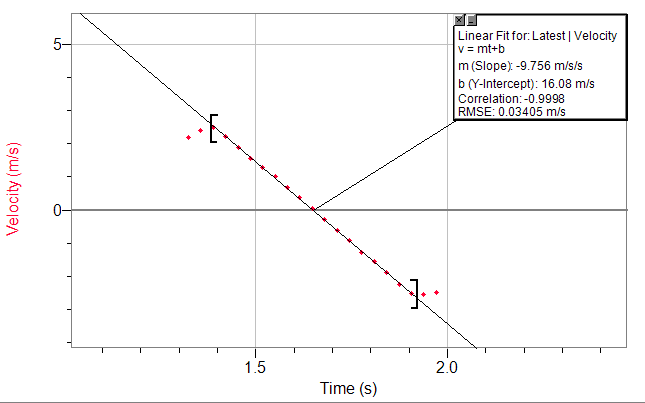
\includegraphics[width=3in]{1d_velo}
            \caption{Y velocity for one bounce of the ball.}
            \label{fig:1d_velo}
        \end{figure}
        \item [3b)] The slope of the graph is acceleration.
        \item [3c)] My value of \SI{-9.76}{\meter\per\second\squared} is fairly close to \SI{-9.81}{\meter\per\second\squared}, but not within error of the linear fit.
        \setcounter{enumi}{3}
        \item \displaystyle\(\Delta x = v_0 t + \frac{1}{2} a t^2\)
        \item The figure shows the distance away from the sensor of the bouncy ball with respect to time.
        The data is very good, given the correlation with the equation and the RMSE being 2 magnitudes smaller than the data.
        \begin{figure}[H]
            \centering
            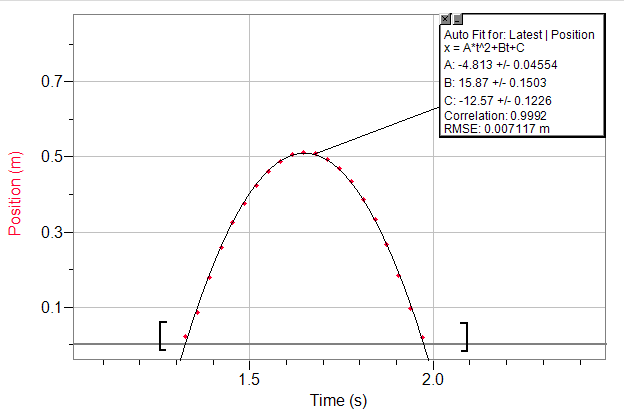
\includegraphics[width=3in,height=1.8in]{1d_pos}
            \caption{Y position for one bounce of the ball.}
            \label{fig:1d_pos}
        \end{figure}
    \end{enumerate}

    \pagebreak


    \section{2D Motion}

    \begin{enumerate}
        \item 2D graphs:
        \begin{figure}[H]
            \begin{subfigure}[t]{0.5\textwidth}
                \centering
                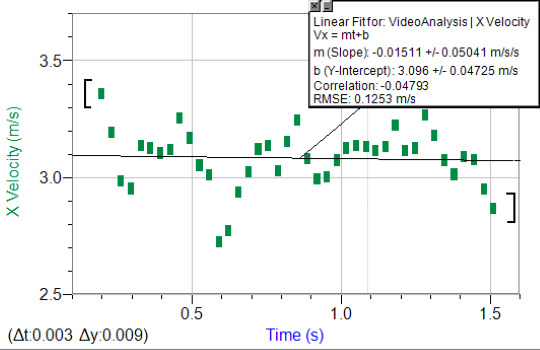
\includegraphics[height=1.7in, width=2.5in]{2d_x_velo_(Custom)}
                \caption{X velocity.}
            \end{subfigure}%
            ~
            \begin{subfigure}[t]{0.5\textwidth}
                \centering
                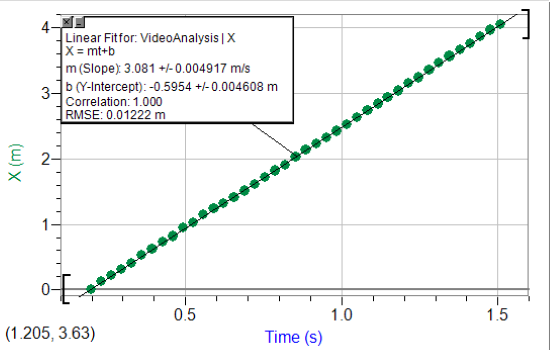
\includegraphics[height=1.7in, width=2.5in]{2d_x_pos_(Custom)}
                \caption{X position.}
            \end{subfigure}
            \caption{X component of basketball motion.}
        \end{figure}

        \begin{figure}[H]
            \begin{subfigure}[t]{0.5\textwidth}
                \centering
                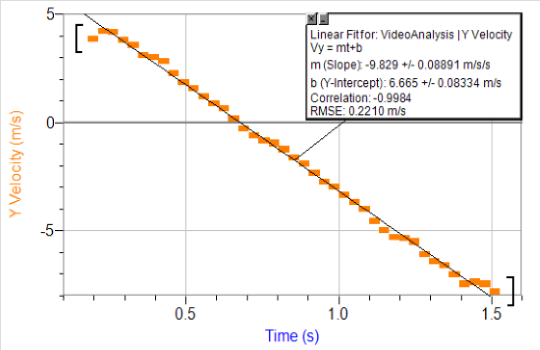
\includegraphics[height=1.7in, width=2.5in]{2d_y_velo_(Custom)}
                \caption{Y velocity.}
            \end{subfigure}%
            ~
            \begin{subfigure}[t]{0.5\textwidth}
                \centering
                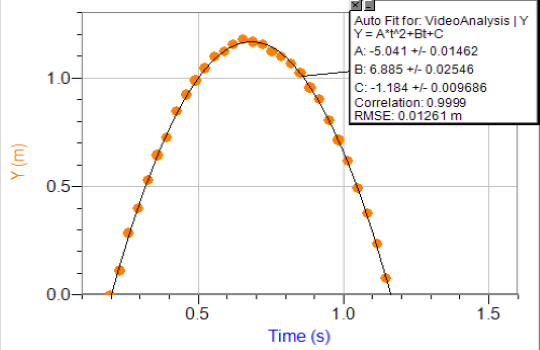
\includegraphics[height=1.7in, width=2.5in]{2d_y_pos_(Custom)_1}
                \caption{Y position}
            \end{subfigure}
            \caption{Y component of basketball motion.}
        \end{figure}
        \item The 5 most important steps are to:
        \begin{enumerate}
            \item Make sure the sensor is parallel to the floor.
            \item Make sure the ball had one good perpendicular bounce.
            \item Make sure my hand was out of the way by the time the sampling started to not block the sensor.
            \item Make sure the ultrasonic sensor is on the correct setting (ball, and not cart).
            \item Make sure there is no initial velocity when dropping the ball.
        \end{enumerate}
        \item Experimental questions:
        \begin{enumerate}
            \item 1D
            \begin{enumerate}
                \item It looks like a parabolic arc.
                \item The velocity is changing and the acceleration is constant.
                The velocity was bounded by about \SI{2.7}{\meter\per\second} and \SI{-2.7}{\meter\per\second} for the duration of the bounce and the acceleration was almost constant \SI{-9.76}{\meter\per\second\squared} due to some imperfections.
                The shape of the velocity graph was sawtooth like, and the acceleration is a flat line.
            \end{enumerate}
            \item 2D
            \begin{enumerate}
                \item The basketball followed a parabolic arc.
                \item The velocity was centered about a constant \SI{3.1}{\meter\per\second}.
                Acceleration was 0.
                They are both lines.
                \item The velocity is changing, acceleration is constant.
                Velocity was from about \SI{4}{\meter\per\second} to \SI{-4}{\meter\per\second}. (LoggerPro added extraneous data past the 1.2 second mark.) The shape of the velocity graph was a decreasing line and acceleration's is a line.
            \end{enumerate}
        \end{enumerate}
        \item A similarity is that both Y position graphs had a parabolic shape.
        A dissimilarity is that the basketball is more conic.
        This is due to the initial velocity imparted by the player, whereas I simply let go of the ball.
    \end{enumerate}

    \pagebreak

    \begin{meme}[t]
        \centering
        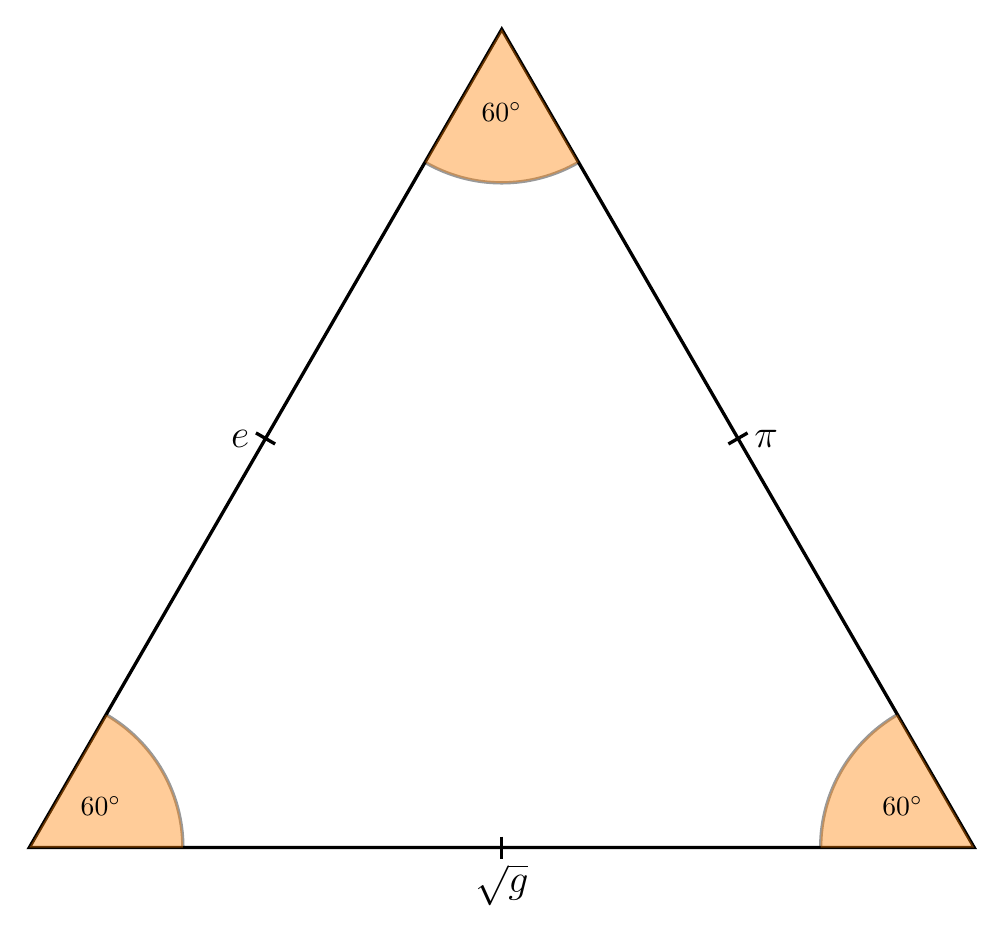
\begin{tikzpicture}[scale=3, very thick]
            \coordinate (O) at (0,0);
            \coordinate (A) at (4,0);
            \coordinate (B) at (2,3.464);
            \draw (O)--(A)--(B)--cycle;

            \tkzLabelSegment[below=2pt](O,A){{\Large$\sqrt{g}$}}
            \tkzLabelSegment[left=2pt](O,B){{\Large$e$}}
            \tkzLabelSegment[right=2pt](A,B){{\Large$\pi$}}

            \tkzMarkSegments[mark=|](O,A O,B A,B)

            \tkzMarkAngle[size=0.65cm,%
                opacity=.4](A,O,B)
            \tkzFillAngle[fill=orange, size=0.65cm,
                opacity=0.4](A,O,B)
            \tkzLabelAngle[pos = 0.35](A,O,B){60\degree}

            \tkzMarkAngle[size=0.65cm,%
                opacity=.4](B,A,O)
            \tkzFillAngle[fill=orange, size=0.65cm,
                opacity=0.4](B,A,O)
            \tkzLabelAngle[pos = 0.35](B,A,O){60\degree}

            \tkzMarkAngle[size=0.65cm,%
                opacity=.4](O,B,A)
            \tkzFillAngle[fill=orange, size=0.65cm,
                opacity=0.4](O,B,A)
            \tkzLabelAngle[pos = 0.35](O,B,A){60\degree}
        \end{tikzpicture}
        \caption{I couldn't think of a Logger Pro meme unfortunately, so have this (admittedly engineering-major-themed) meme instead. ``\ldots by Carlos Medina,'' if you decide to post it.}
    \end{meme}
\end{document}